\section{Results}\label{sec:results}

All numbers in this section are held-out: \nm{B-records} frozen points of comparison (B) and
\nm{A-records} points of comparison (A), over five CPUs, seven sets and three models. A ratio is always
\emph{rival time / our time}, the median over rounds of each divided; above 1 our cascade is faster.
Its 95\% interval comes from a bootstrap over rounds (\S\ref{sec:timing}).

\subsection{Comparison (A): generators under a common rescoring procedure}

\paragraph{One budget, one model per set kind.} Table~\ref{tab:compA-intel} and Figure~\ref{fig:compA}
show the generators at $C = 400$, $H = 100$, each at its smaller declared effort, with CodeRankEmbed on
the code sets and bge-base-en-v1.5 on the BEIR sets. Under the same int8 screen and the same float16
rescoring, retained quality depends on the generator only through its 400 candidates. In this slice,
every graph generator and every flat scan keeps at least 98.4\% of exact quality on every set and CPU
(our walk 99.3\%, our scan 99.7\%, FAISS binary HNSW 98.7\%, USearch b1 98.4\% at their lowest). The
two partition generators do not at their smaller effort: FAISS RaBitQ-IVF keeps 57--92\% and ScaNN
23--100\% of exact quality. Among the generators that keep at least 99\%, one of our two generators is
the fastest in all \nm{A-oursbest} of \nm{A-n} (CPU, set) cells, and the next such generator takes
\nm{A-min} to \nm{A-max} times as long (geometric mean \nm{A-gm}).

\paragraph{Every model, budget and effort.} Over the full grid (\nm{Aall-n} cells of CPU, set, model and
budget in which at least one generator keeps 99\%), whenever one of our generators keeps 99\%, it is the
fastest generator that does ($\nm{Aall-exc}$ exceptions). In \nm{Aall-noours} cells, however, only rival
generators keep 99\%: \nm{Aonly-small} of the \nm{Atot-small} cells with $C \le 200$, \nm{Aonly-400} of
\nm{Atot-400} at $C = 400$ and \nm{Aonly-1000} of \nm{Atot-1000} at $C = 1000$. Most of them pair a code
set with bge-base-en-v1.5, or FiQA with CodeRankEmbed. There the 512-bit sign codes rank the true
neighbours too low for a small candidate budget, and the float32 graphs (hnswlib, FAISS HNSW), whose
candidates come from full-precision distances, keep 99\% where ours do not. Across the full grid, the
lowest retained quality at $C = 400$, $H = 100$ is \nm{Aall-min-ours_walk}\% for our walk,
\nm{Aall-min-ours_scan}\% for our scan, \nm{Aall-min-faiss_bin_hnsw}\% for FAISS binary HNSW,
\nm{Aall-min-hnswlib_f32}\% for hnswlib and \nm{Aall-min-scann}\% for ScaNN.

\paragraph{Generator speed.} Our exact scan is the faster of our two generators up to 22k vectors on
every CPU (the walk takes 1.2--1.6 times as long). On FiQA and dall the walk is faster on the x86 CPUs
and the Mac (0.6--0.9 of the scan's time) and slower on Graviton (1.4 times); above 150k vectors only
the walk runs. The rival binary graphs (FAISS binary HNSW, USearch b1) take 1.9--7.3 times as long as
our walk at the same budget. Their graphs are built with $M = 32$ and ours with $M = 64$, and our walk
adapts its effort per query (\S\ref{sec:compA}), so this is a comparison of the generators as built
and configured here, not of graph search at equal effort. Its cause inside each library is not
established.

\paragraph{The int8 screen.} With our walk at $C = 400$, rescoring all 400 candidates ($H = C$, no
screen) takes a median \nm{screen-med} times as long as screening to $H = 100$ (10th--90th percentile
\nm{screen-p10}--\nm{screen-p90} over \nm{screen-n} CPU--set--model--effort cells), and retained quality
changes by \nm{screen-qmin} to \nm{screen-qmax}.

\begin{figure}[t]\centering
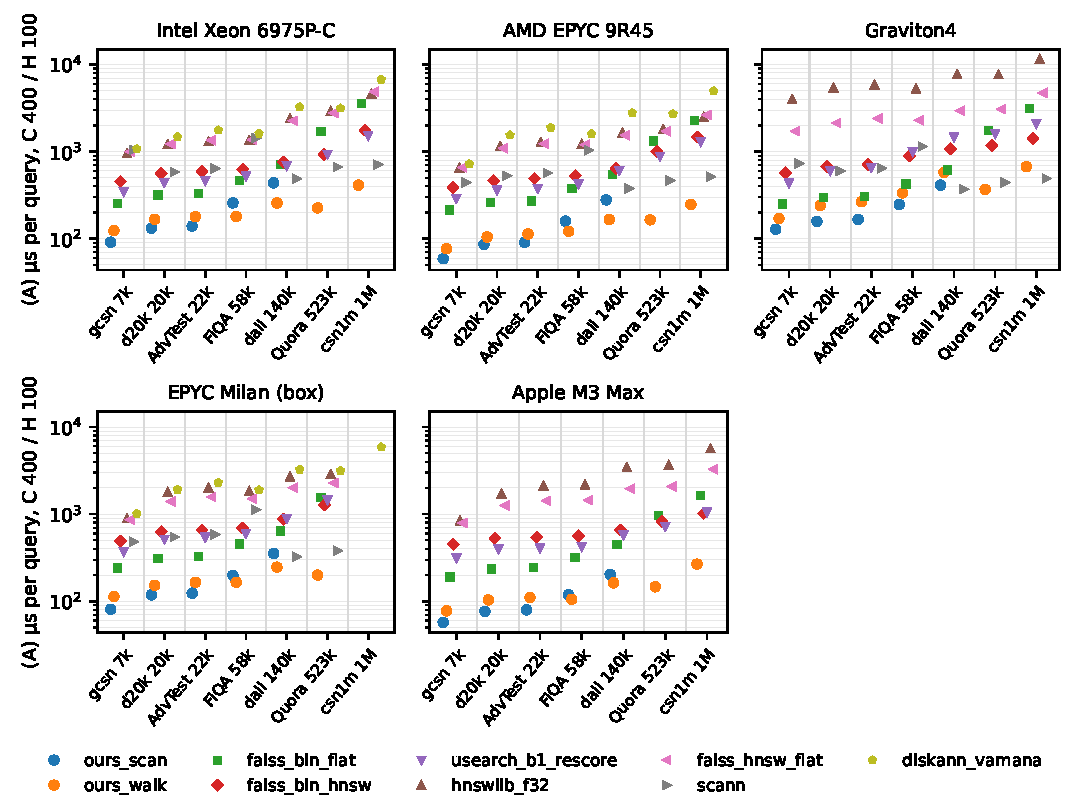
\includegraphics[width=\textwidth]{figures/compA.pdf}
\caption{Comparison (A), held-out, per CPU: \us{} per query of each plotted generator plus the shared
int8 screen and rescoring, at $C = 400$, $H = 100$, smaller declared effort, against corpus size,
with CodeRankEmbed (code sets) and bge-base-en-v1.5 (BEIR sets). FAISS RaBitQ flat and IVF are in the
tables only. Retained quality per cell is in Tables~\ref{tab:compA-intel}--\ref{tab:compA-mac}.}\label{fig:compA}
\end{figure}

\compAtable{intel}{Intel Xeon 6975P-C}

\subsection{Comparison (B): as shipped, at the same retained quality}

Table~\ref{tab:headline099} compares our cascade with the rival that was fastest \emph{on dev} at
$\fr = 0.99$, each at its frozen point; held-out data decide nothing about which rival is shown. The
table marks where our point ($\dagger$) or the rival's ($\ddagger$) misses $\fr$ on held-out by its point
estimate. Figure~\ref{fig:size} plots our cascade against corpus size. On these sets, the ratio
depends on corpus size more than on the CPU.

\begin{itemize}\setlength{\itemsep}{1pt}
\item \textbf{Large sets} (Quora, 523k vectors; csn1m, 1M): ours is faster in \nm{faster-large} of
\nm{n-large} cells (whole interval above 1) and slower in \nm{slower-large}; ratios \nm{min-large} to
\nm{max-large}, geometric mean \nm{gm-large}. The rivals here are graph indexes: FAISS HNSW (float32,
SQ8, binary or RaBitQ codes), USearch b1, and SVS Vamana with LVQ or LeanVec on Intel. Several large-set
intervals are wide because of slow rounds of our cascade (\S\ref{sec:losses}).
\item \textbf{Middle sets} (FiQA, 58k; dall, 140k): mixed. Ours is faster in \nm{faster-mid} of
\nm{n-mid} cells and slower in \nm{slower-mid} (geometric mean \nm{gm-mid}).
\item \textbf{Small code sets} (gcsn, d20k, AdvTest; 7k--22k): the rivals are faster in most cells. Ours
is slower in \nm{slower-small} of \nm{n-small} cells and faster in \nm{faster-small} (geometric mean
\nm{gm-small}). The rival is usually FAISS binary flat: an exact Hamming scan of the same 512-bit codes,
followed by float refine, in C++.
\end{itemize}

Over all CPUs and sets, the geometric mean of the ratio at $\fr = 0.99$ is \nm{gm-all-099}
(\nm{gmn-all-099} cells, ours faster by point estimate in \nm{wins-all-099}); per CPU it is
\nm{gm-intel-099} (Intel), \nm{gm-amd-099} (AMD), \nm{gm-arm-099} (Graviton), \nm{gm-box-099} (box,
reduced grid) and \nm{gm-mac-099} (Mac, reduced grid). At $\fr = 0.995$ it is \nm{gm-all-0995}
(Appendix~\ref{app:fractions}). The four code sets gcsn, d20k, dall and csn1m share one query set, so
their cells are four sizes of one test, not four independent tests; the geometric means are descriptive.
The large sets are mostly faster and the small code sets mostly slower on every CPU, while some middle
cells change sign between CPUs (FiQA with bge: 0.88 on Intel, 0.69 on AMD, 1.41 on Graviton).

\headlinetable{0.99}{099}

\begin{figure}[t]\centering
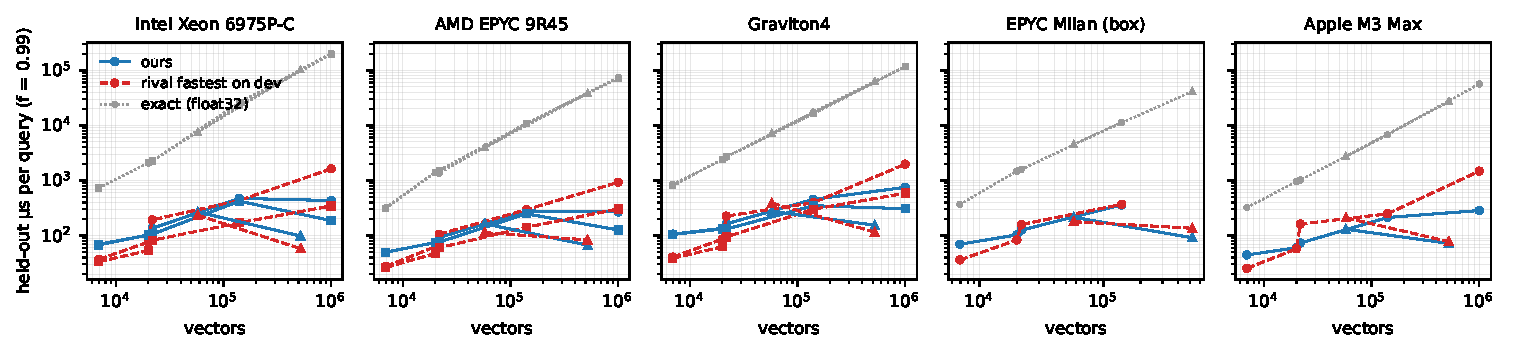
\includegraphics[width=\textwidth]{figures/size.pdf}
\caption{Comparison (B), held-out, $\fr = 0.99$, per CPU: our cascade (blue), the rival that was fastest on dev
at $\fr$ (red, dashed; Table~\ref{tab:headline099}) and exact float32 search (grey), against corpus size. Circles and squares: code sets with CodeRankEmbed and
jina; triangles: BEIR sets with bge-base-en-v1.5.}\label{fig:size}
\end{figure}

\paragraph{Held-out re-test of the dev points.} Every frozen point met its fraction on dev with the
one-sided 97.5\% bound. On held-out queries at $\fr = 0.99$, all \nm{ret-ours-n} of our points meet it by
the point estimate and \nm{ret-ours-bound} (\nm{ret-ours-boundpct}\%) by the bound; of the
\nm{ret-riv-n} rival points, \nm{ret-riv-point} (\nm{ret-riv-pointpct}\%) meet it by the point estimate
and \nm{ret-riv-bound} (\nm{ret-riv-boundpct}\%) by the bound. A point chosen as the fastest that passes
on dev sits close to the boundary, so a fresh sample moves it either way; we report the re-test and do
not re-select.

\paragraph{Tuning budget.} The dev selection gave each system its own declared grid
(Table~\ref{tab:tuning}): up to \nm{tune-max} configurations per set and model for the graph families
with refine, and \nm{tune-ours} for our cascade. Our production defaults were tuned earlier on the gcsn
dev queries, outside this study.

\begin{table}[t]\centering\scriptsize
\caption{Tuning budget: distinct comparison-(B) configurations per set and model in the dev sweep
(including the widened IVF and ScaNN grids), per AWS CPU. Empty: the system does not run on that CPU.}\label{tab:tuning}
\begin{tabular}{lrrr}\toprule
System & Intel & AMD & Graviton\\\midrule
\inputtable{tables/tuning.tex}
\bottomrule\end{tabular}
\end{table}

\paragraph{Hamming ties (dev only).} Sign codes produce many equal Hamming distances. On gcsn dev with
CodeRankEmbed, the run of tied candidates crosses the stage-1 cut at $C = 400$ on 97.8\% of queries;
changing the order inside tie runs changes the retained candidate set on about 28\% of queries, the
top-10 documents on about 1.6\%, and MRR@10 by at most 0.0001 over five random tie orders. This analysis
ran on dev before the freeze, with vectors from an earlier embedding run of the same model.

\subsection{Primary comparisons}

Table~\ref{tab:primary} gives the \nm{nprimary} primary pairs. Following the plan, a pair whose power
on dev was below 0.8 is reported descriptively: \nm{ndescr} pairs (FiQA with bge-base-en-v1.5 on AMD and
Graviton). Quality non-inferiority at $\delta = \nm{delta}$ passes in \nm{nprimarypass} of the
\nm{nconfirm} confirmatory pairs after Holm; the failure is FiQA with bge-base-en-v1.5 on Intel
(observed difference $-0.0015$, 259 held-out queries). On latency, which is descriptive, ours is faster in
\nm{nprimaryfaster} pairs and slower in \nm{nprimaryslower} (whole interval on one side of 1). Two of the
slower pairs compare against a rival point that misses $\fr$ on held-out (FiQA with jina: SVS LVQ on
Intel and hnswlib on AMD), so they are not at matched quality.

\begin{table}[t]\centering\scriptsize
\caption{Primary pairs (fixed on dev; $\fr = 0.99$, comparison B). Ratio: rival / our latency (median over
rounds, 95\% bootstrap interval over rounds). Meets: point estimate / bound, for ours ; rival. Quality:
mean of per-query nDCG@10 (ours $-$ rival) and its one-sided 97.5\% lower bound; non-inferiority at
$\delta = \nm{delta}$, Holm over the \nm{nconfirm} confirmatory pairs; descr.: power below 0.8 on dev,
descriptive.}\label{tab:primary}
\setlength{\tabcolsep}{3pt}
\begin{tabular}{llllrlrrrl}\toprule
CPU & Set & Model & Rival & Ratio & Meets & Mean diff & Lower & $p$ & Holm\\\midrule
\inputtable{tables/primary.tex}
\bottomrule\end{tabular}
\end{table}

\subsection{Memory, load and build}

Table~\ref{tab:mem-csn1m} shows memory and cold start at 1M vectors on the Linux machines (Quora and dall
in Appendix~\ref{app:mem}). Our cascade holds the graph, the codes, the int8 rows and the float16
vectors, memory-mapped from its index files, plus the Node.js runtime: \nm{mem-ours-intel}~GiB on Intel
(\nm{mem-ours-amd} on AMD, \nm{mem-ours-arm} on Graviton), more than \nm{mem-smaller-intel} of the
\nm{mem-nriv-intel} rival points on Intel. The smallest is USearch int8 at \nm{mem-rivalmin-intel}~GiB;
the rivals that refine with float32 originals use 3.0--3.6~GiB, and FAISS HNSW-SQ8
\nm{mem-rivalmax-intel}~GiB. Our cold start (load plus first query after the page cache is dropped) is
\nm{cold-ours-intel}~s on Intel against \nm{cold-rivalmin-intel}--\nm{cold-rivalmax-intel}~s for the
rivals; the rival numbers include the harness's buffered read of the originals (\S\ref{sec:systems}), so
this comparison is indicative. Table~\ref{tab:build} lists build cost at 1M: our build took
\nm{build-ours-s}~s (\nm{build-ours-h}~hours) of wall time on one thread with a peak of
\nm{build-ours-peak}~GB, the longest wall time of any build (the longest rival build took
\nm{build-rival-max-s}~s on 16 threads). In core-seconds our build is below the largest rival graph
builds.

\memtable{csn1m}{csn1m, CodeRankEmbed}

\begin{table}[t]\centering\scriptsize
\caption{Build cost at 1M vectors (csn1m, CodeRankEmbed), one row per family: the range over its
build grid. Builds ran under a memory-admission scheduler, several at a time, so wall times are
indicative. Core-seconds = wall time $\times$ threads (an upper bound for the concurrent rival builds).}\label{tab:build}
\begin{tabular}{lrrrrrr}\toprule
Family & Builds & Wall s & Threads & Core-s & Size GB & Peak RSS GB\\\midrule
\inputtable{tables/build.tex}
\bottomrule\end{tabular}
\end{table}
